\chapter{\label{cha:sts_state_of_the_art_methods}State of the Art Methods}

The biggest challenge that the neural based architectures face when applied to STS tasks is the small size of datasets available to train them. As a result, in many cases the networks cannot be trained properly. Given the amount of human labour required to produce datasets for STS, it is not possible to have high quality large training datasets. As a result researches working in the field have also considered unsupervised methods for STS. Recent unsupervised approaches use pretrained word/sentence embeddings directly for the similarity task without training a neural network model on them. Such approaches have used cosine similarity on sent2vec \cite{pagliardini-etal-2018-unsupervised}, InferSent \cite{conneau-EtAl:2017:EMNLP2017}, Word Mover's Distance \cite{10.5555/3045118.3045221}, Doc2Vec \cite{10.5555/3044805.3045025} and Smooth Inverse Frequency with GloVe vectors \cite{DBLP:conf/iclr/AroraLM17}. While these approaches have produced decent results in the final rankings of shared tasks, they have also provided strong baselines for the STS task. 

This chapter explores the performance of three unsupervised STS methods - cosine similarity using average vectors, Word Mover's Distance \cite{10.5555/3045118.3045221} and cosine similarity using Smooth Inverse Frequency \cite{DBLP:conf/iclr/AroraLM17} and how to improve them using contextual word embeddings which will be explained more in Section \ref{sec:state_related}. The main contributions of this part of the thesis are as follows.

\begin{enumerate}
	\item In the Related Work Section (Section \ref{sec:state_related}), we cover three unsupervised STS techniques to compute semantic similarity at the sentence level. 
	
	\item We propose an improved unsupervised STS method based on contextual word embeddings. 
	
	\item The code with the experiments conducted will be publicly available to the community\footnote{The public GitHub repository is available on \url{https://github.com/tharindudr/simple-sentence-similarity}}.
	
	\item We published the findings in this chapter in \citet{ranasinghe-etal-2019-enhancing}.
	
\end{enumerate}

The rest of this chapter is organised as follows. Section \ref{sec:state_related} describes the three unsupervised STS methods we experimented in this section. In section \ref{sec:state_method} we present the methodology, the contextual word embeddings we used followed by the results to the English datasets comparing with the baselines. Section \ref{sec:state_languages} and Section \ref{sec:state_domains} shows how our method can be applied to different languages and domains and their results. The chapter finishes with conclusions and ideas for future research directions in unsupervised STS methods.


\section{Related Work}
\label{sec:state_related}
Given that a good STS metric is required for a variety of natural language processing fields, researchers have proposed a large number of such metrics. Before the shift of interest in neural networks, most of the proposed methods relied heavily on feature engineering. With the introduction of word embedding models, researchers focused more on neural representation for this task. The three unsupervised STS methods explored in this paper: Cosine similarity on average vectors, Word Mover's Distance and Cosine similarity using Smooth Inverse Frequency are the most common unsupervised methods explored in STS tasks. Apart from them cosine similarity of the output from Infersent \cite{Conneau2017SupervisedLO}, sent2vec \cite{Pagliardini2018UnsupervisedLO} and doc2vec \cite{Le2014DistributedRO} have been used to represent the similarity between two sentences which we discuss in the next chapter. 


\subsection{Cosine Similarity on Average Vectors}
The first unsupervised STS method that we used to estimate the semantic similarity between a pair of sentences, takes the average of the word embeddings of all words in the two sentences, and calculates the cosine similarity between the resulting embeddings. This is a common way to acquire sentence embeddings from word embeddings. Obviously, this simple baseline leaves considerable room for variation. Researches have investigated the effects of ignoring stopwords and computing an average weighted by tf-idf in particular.

\subsection{Word Mover's Distance}
The second STS state of the arts method that we have considered is Word Mover's Distance introduced by \citet{10.5555/3045118.3045221}. Word Mover's Distance uses the word embeddings of the words in two texts to measure the minimum distance that the words in one text need to ``travel'' in semantic space to reach the words in the other text as shown in Figure \ref{fig:WMD}. \citet{10.5555/3045118.3045221} says that this is a good approach than vector averaging since this technique keeps the word vectors as it is through out the operation. We have investigated the effects of considering/ ignoring stop words before calculating the word mover's distance.

\begin{figure}[ht]
	\centering
	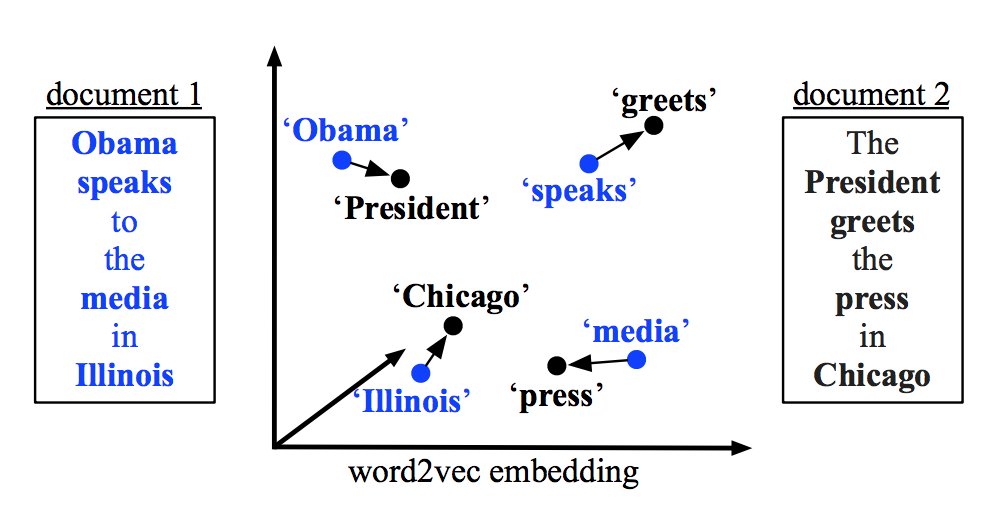
\includegraphics[scale=0.4]{figures/semantic_textual_similarity/state_of_the_art/word_movers_distance.png}
	\caption{The Word Mover's Distance between two sentences}
	\label{fig:WMD}
\end{figure}

\subsection{Cosine Similarity Using Smooth Inverse Frequency}
The third and the last unsupervised STS method we have considered is to acquire sentence embeddings using Smooth Inverse Frequency proposed by \citet{DBLP:conf/iclr/AroraLM17} and then calculate the cosine similarity between those sentence embeddings. Semantically speaking, taking the average of the word embeddings in a sentence tends to give too much weight to words that are quite irrelevant. Smooth Inverse Frequency tries to solve this problem in two steps. 

\begin{enumerate}
	\item Weighting: Smooth Inverse Frequency takes the weighted average of the word embeddings in the sentence. Every word embedding is weighted by $a\over{a + p(w)}$, where $a$ is a parameter that is typically set to 0.001 and $p(w)$ is the estimated frequency of the word in a reference corpus. 
	\item Common component removal: After that, Smooth Inverse Frequency computes the principal component of the resulting embeddings for a set of sentences. It then subtracts their projections on first principal component from these sentence embeddings. This should remove variation related to frequency and syntax that is less relevant semantically.
\end{enumerate}

As a result, Smooth Inverse Frequency downgrades unimportant words such as \emph{but, just}, etc., and keeps the information that contributes most to the semantics of the sentence. After acquiring the sentence embeddings for a pair of sentences, the cosine similarity between those two vectors were taken to represent the similarity between them. 

All of these STS methods are based on word embeddings/vectors. The main weakness of word vectors is that each word has the same unique vector regardless of the context it appears. For an example, the word "play" has several meanings, but in standard word embeddings such as GloVe \cite{pennington2014glove}, FastText \cite{mikolov-etal-2018-advances} or Word2Vec  \cite{10.5555/2999792.2999959} each instance of the word has the same representation regardless of the meaning which is used. As an example the word 'bank' in two sentences - ``I am walking by the river bank'' and ``I deposited money to the bank'' would have the same embeddings which can be confusing for machine learning models. The recent introduction of contextualised word representations solved this problem by providing vectors for words considering their context too. In this way the word 'bank' in above sentences have two different embeddings. Therefore, we explore how the contextualised word representations can improve the above mentioned unsupervised STS methods. The following contextualised word representation models were considered for the experiments. We will explain the neural network architectures of these contextual word embeddings in Chapter \ref{cha:sts_transformers}. For this chapter, we considered these architectures as a black box where we just feed the words to get the embeddings. We considered these contextualised word representations mainly considering the popularity they had by the time we were doing the experiments.

\begin{enumerate}
\item \textbf{ELMo\footnote{More details about ELMo can be viewed on \url{https://allennlp.org/elmo}}}
introduced by \citet{peters-etal-2018-deep} use bidirectional language model (biLM) to learn both word (e.g., syntax and semantics) and linguistic context. After pre-training, an internal state of vectors can be transferred to downstream natural language processing tasks. ELMo vectors have been successfully used many natural language processing tasks like text classification \cite{jiang-etal-2019-team}, named entity recognition \cite{Luo2018} which motivated us to explore ELMo in unsupervised STS methods. Also, we were aware about the fact that ELMo has been pre-trained on different languages \cite{che-EtAl:2018:K18-2} and different domains \cite{jin2019probing} which will be easier when we are adopting our methodology for different languages and domains in Sections \ref{sec:state_languages} and \ref{sec:state_domains}.

\item \textbf{BERT\footnote{The GitHub repository of BERT is available on \url{https://github.com/google-research/bert}}} introduced by \citet{devlin-etal-2019-bert} might probably be the most popular contextualised word embedding model. In contrast to ELMo which uses a shallow concatenation layer \cite{devlin-etal-2019-bert}, BERT employs a deep concatenation layer. As a result BERT is considered a very powerful embedding architecture. BERT has been successfully applied in many natural language processing tasks like text classification \cite{Ranasinghe2019a}, word similarity \cite{hettiarachchi-etal-2020-brums}, named entity recognition \cite{10.1145/3394486.3403149}, question and answering \cite{yang-etal-2019-end} etc. Similar to ELMo, BERT too has been widely adopted to different languages such as Arabic \cite{antoun-etal-2020-arabert}, French \cite{martin-etal-2020-camembert} etc. and different domains such as SciBERT \cite{beltagy-etal-2019-scibert} and BioBERT \cite{10.1093/bioinformatics/btz682} etc.  

\item \textbf{Flair\footnote{The GitHub repository of Flair is available on \url{https://github.com/flairNLP/flair}}} is another type of popular contextualised word embeddings introduced in \citet{akbik-etal-2018-contextual}. It takes a different approach by using a character level language model rather than the word level language model used in ELMo and BERT. Flair also has been used successfully in natural language processing tasks such as named entity recognition \cite{akbik-etal-2019-pooled}, part-of-speech tagging \cite{akbik-etal-2018-contextual} and has been widely adopted in to different languages and domains \cite{akbik-etal-2018-contextual,sharma2019bioflair}.

\end{enumerate}

Apart from using these contextual word embedding models individually we also considered \textbf{Stacked Embeddings} of these models together. Stacked Embeddings are obtained by concatenating different embeddings. According to \citet{akbik-etal-2018-contextual} stacking the embeddings can provide a powerful embeddings to represent words. Therefore, we experimented with several combinations of Stacked Embeddings.

Even though these contextual word embedding models have shown promising results in many natural language processing tasks, to the best of our knowledge none of these contextual word representations has been applied on unsupervised STS methods.  



\section{Improving State of the Art STS Methods}
\label{sec:state_method}
As mentioned before we applied different contextual word embeddings on three unsupervised STS methods and their variants. First we experimented with English STS datasets we explained in Section \ref{sec:sts_intro_datsets}. Our implementation was based on \textit{Flair-NLP} Framework \cite{akbik-etal-2019-flair} which makes it easier to switch between different word embedding models when acquiring word embeddings. Also \textit{Flair-NLP} has their own model zoo of pre-trained models to allow researchers to use state-of-the-art NLP models in their applications. For English, all of these contextualised word embedding models come with different variants like \textit{small, large etc.}. Usually the larger models provide a better accuracy since they have been trained on a bigger dataset compared to the smaller models. However, this comes with the disadvantage that these larger models are resource-intensive than the smaller models. In order to achieve a better accuracy, we used the largest model available in each contextual word embedding models. We will describe them in the following paragraphs. 

For ELMo we used the 'original (5.5B)' pre-trained model provided in \citet{peters-etal-2018-deep} which was trained on a dataset of 5.5B tokens consisting of Wikipedia (1.9B) and all of the monolingual news crawl data from WMT\footnote{WMT: Workshop on Statistical Machine Translation is a leading conference in NLP that is being organised annually.} 2008-2012 (3.6B). \citet{peters-etal-2018-deep} mentions that ELMo original (5.5B) has slightly higher performance than other ELMo models and recommend it as a default model. Using this model we represented each word as a vector with a size of 3072 values.

For BERT we used the 'bert-large-cased' pre-trained model. Compared to the 'bert-base-cased' model, this model provided slightly better results in all the NLP tasks experimented in \citet{devlin-etal-2019-bert}. We represented each word as a 4096 lengthened vector using this model. 

As suggested in \citet{akbik-etal-2018-contextual} the recommended way to use Flair embeddings is to stack pre-trained 'news-forward' flair embeddings and pre-trained flair 'news-backward' embeddings with GloVe \cite{pennington-etal-2014-glove} word embeddings. We used the stacked model to represent each word as a 4196 lengthened vector. 

In the following list we show the performance of each unsupervised STS method with contextual word embeddings on different English STS datasets. 

\begin{enumerate}
	\item \textbf{Cosine Similarity on Average Vectors} - The first unsupervised STS method we tried to improve using contextual word embeddings is Cosine Similarity on Average Vectors which we explained on Section \ref{sec:state_related}.
\end{enumerate}







\section{Portability to Other Languages}
\label{sec:state_languages}

\section{Portability to Other Domains}
\label{sec:state_domains}

\section{Conclusions}